\lstinputlisting[style=cstyle]{Questions/Part3/prime3.c}

\subsubsection*{\underline{Experimental}}

\begin{tabular}{|c|c|c|c|c|c|c|c|c|c|c|}
\hline
N & 1000003 & 2000003 & 4000037 & 8000009 & 16000057 & 32000011 & 64000031 & 128000003 & 256000001 & 512000009 \\
\hline
\makecell{T(n)\\\(10^{-5}\)} & 7.5 & 7.6 & 7.7 & 8.2 & 8.8 & 9.2 & 11.4 & 12 & 14.6 & 17\\
\hline
\end{tabular}

\vspace{0.25cm}

\begin{tabular}{|c|c|c|}
    \hline
    N & 1024000009 & 2048000011\\
    \hline
    \makecell{T(n)\\\(10^{-5}\)}  & 25.3 & 26.5\\
    \hline
\end{tabular}

\vspace{0.5cm}

\begin{figure}[h!]
    \centering
    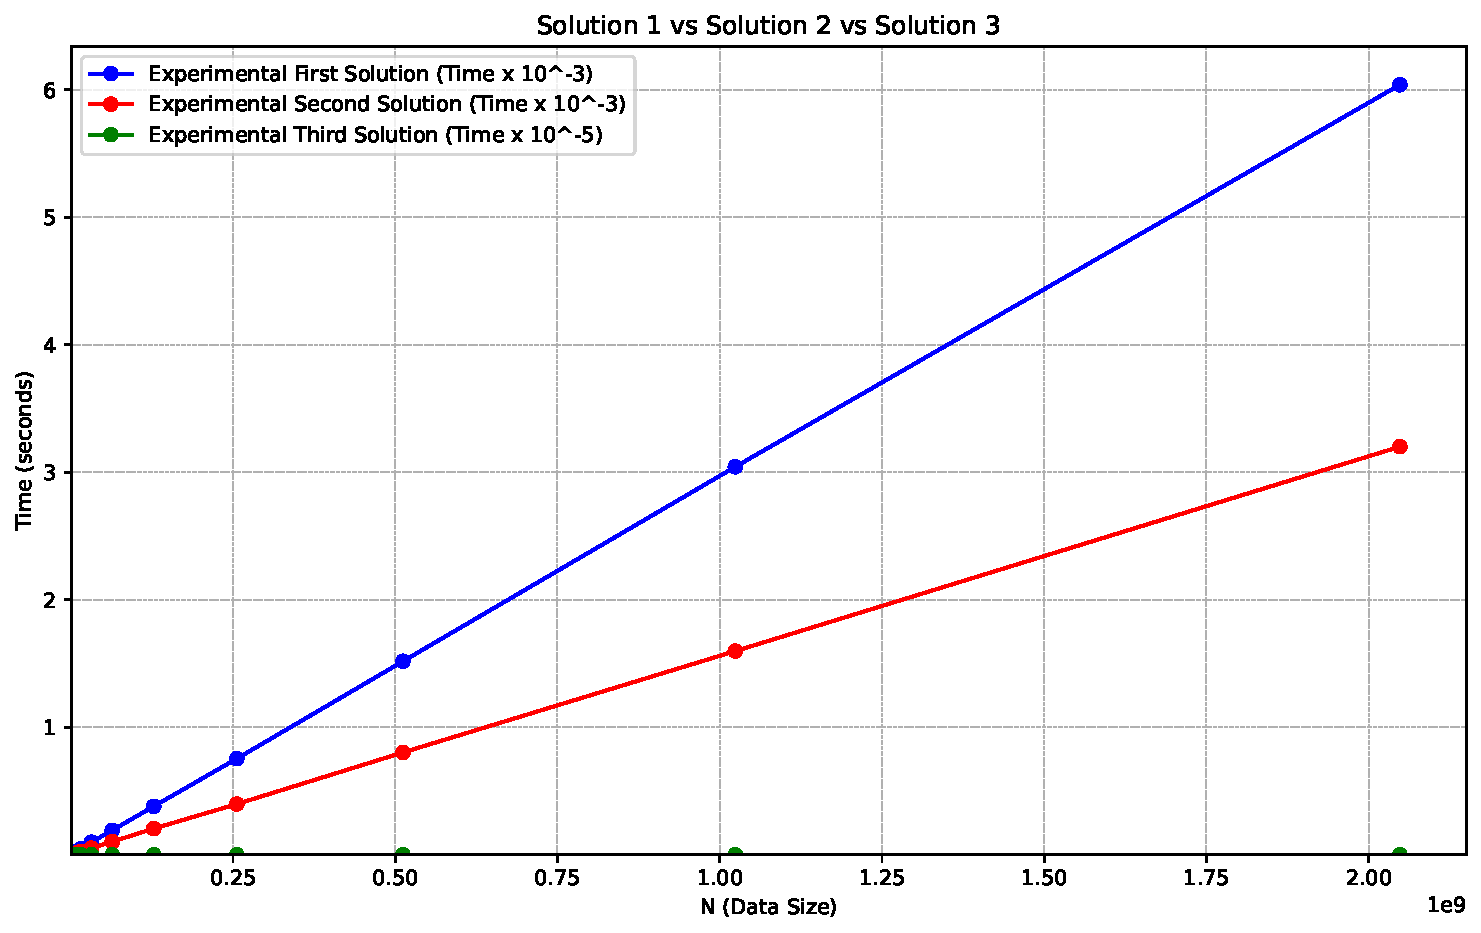
\includegraphics[width=0.85\textwidth]{Questions/Part3/plot.pdf}
    \label{fig:time_plot}
\end{figure}

\newpage

To Draw the plots i used the below python script :

\vspace{1cm}

\lstinputlisting[style=pythonstyle2,inputencoding=utf8]{Questions/Part3/draw.py}

\vspace{1cm}

\begin{prettyBox}{Observation}{greenPlot}
We notice in the plots that the green plot (the 3rd solution plot) is barely visible due to its y range of values
being much smaller than the red and blue (solution 1 and 2) , so the third solution is the most efficient of them 
\end{prettyBox}

\newpage

\begin{figure}[h!]
    \centering
    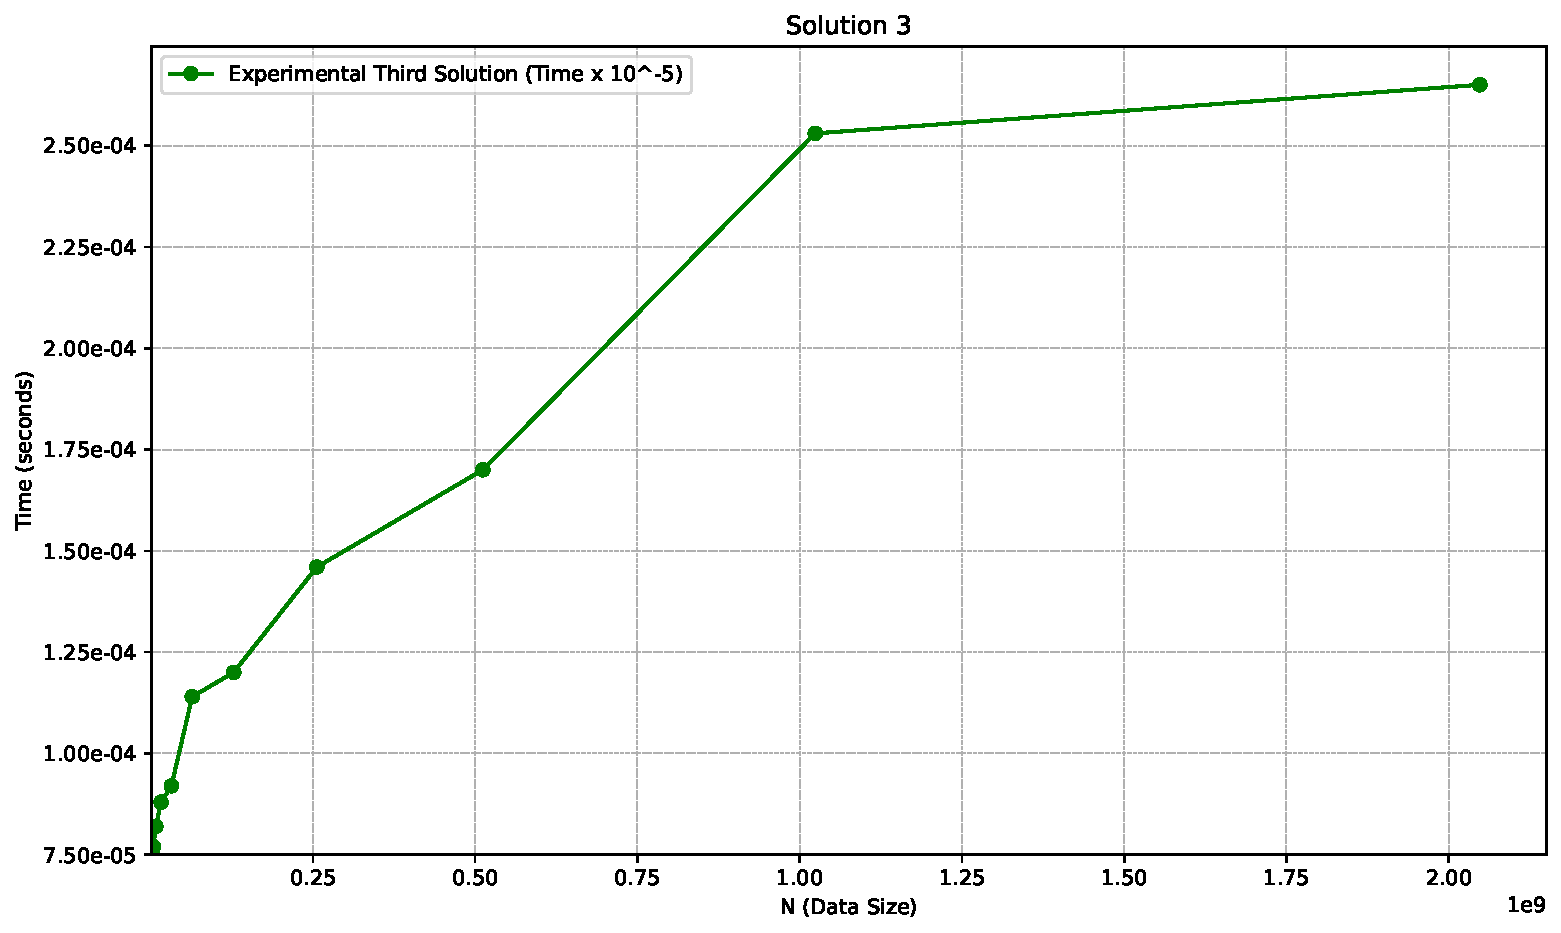
\includegraphics[width=0.85\textwidth]{Questions/Part3/sqrt.pdf}
    \label{fig:time_plot}
\end{figure}

\newpage

To Draw the plot i used the below python script :

\vspace{1cm}

\lstinputlisting[style=pythonstyle2,inputencoding=utf8]{Questions/Part3/drawsqrt.py}


